\documentclass[../TDO1-O2.tex]{subfiles}%

\begin{document}
\section[s]"1"{Détermination directe de l'indice d'un liquide}

\QR{%
	~
	\smallbreak
	\vspace{-28pt}
	\noindent
	\begin{isd}[lefthand ratio=.68, interior hidden]
		Un rayon lumineux dans l'air ($n_{\rm air}$) tombe sur la surface
		horizontale d'un liquide d'indice $n$. Il fait un angle $\alpha =
			\ang{56;;}$ avec le plan horizontal. La déviation entre le rayon incident et
		le rayon réfracté est $D = \ang{13.5;;}$. Quel est l'indice $n$ du liquide~?
		\tcblower
		\begin{center}
			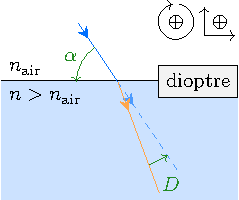
\includegraphics[width=\linewidth]{dioptre_alpha-horiz_plain}
			\label{fig:alpha_horiz}
		\end{center}
	\end{isd}
	\vspace{-30pt}
}{%
	Cet exercice est d'une simplicité absolue. Et pourtant…
	\begin{tcn}[sidebyside, righthand ratio=.45](data){Données}
		\begin{enumerate}
			\item Rayon incident sur un dioptre entre air et milieu d'indice $n$ :
			      angle {\huge avec le dioptre} de \ang{56;;} ;
			\item Différence d'angle entre rayon incident et réfléchi (« déviation
			      ») de \ang{13.5;;}.
		\end{enumerate}
		\tcblower
		\begin{center}
			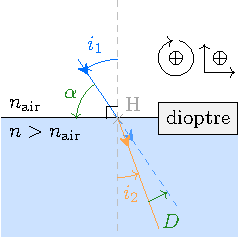
\includegraphics[width=5cm]{dioptre_alpha-horiz.pdf}
		\end{center}
	\end{tcn}
	\begin{tcbraster}[raster columns=6, raster equal height=rows]
		\begin{tcn}[raster multicolumn=2](ques){Résultat attendu}
			Indice du liquide.
		\end{tcn}
		\begin{tcn}[raster multicolumn=4](tool)'r'{Outils du cours}
			Loi de \textsc{Snell-Descartes}~:
			\[
				\boxed{n_1\sin i_1 = n_2 \sin i_2}
			\]
			avec $n_1$ l'indice du milieu d'incidence, $n_2$ celui du milieu de
			réfraction, $i_1$ l'angle d'incidence et $i_2$ l'angle de réfraction.
		\end{tcn}
	\end{tcbraster}

	\begin{tcn}(appl){Application}
		Un bon schéma fait attentivement est \textbf{nécessaire} ici. En effet,
		les angles donnés ne sont pas ceux qu'on utilise dans la relation de
		\textsc{Snell-Descartes}. \bigbreak

		En appelant $\alpha$ l'angle entre le rayon et le dioptre, on a
		\[ \alpha + i_1 = \ang{90;;}\]
		donc \fbox{$i_1 = \ang{34;;}$}. Et en appelant $D$ la déviation entre
		les deux rayons, on a
		\[ i_1 = i_2 + D\]
		soit \fbox{$i_2 = \ang{20.5;;}$}. On en déduit donc
		\[\boxed{n = \frac{\sin i_1}{\sin i_2}} \quad \text{avec} \quad
			\left\{
			\begin{array}{rcl}
				i_1 & = & \ang{34;;}   \\
				i_2 & = & \ang{20.5;;}
			\end{array}
			\right. \quad \text{soit} \quad \boxed{n = 1.6}
		\]
	\end{tcn}
}

\end{document}
